\documentclass[twocolumn,a4paper]{IEEEtranfr}
\usepackage{verbatim}
\usepackage{graphicx}
\usepackage{algorithm}
\usepackage{algorithmic}
\usepackage{listings}
\usepackage{url}
% français
\usepackage[french]{babel}
% accents
\usepackage{ucs}
\usepackage[utf8x]{inputenc}
%\usepackage[T1]{fontenc}
\usepackage{subfigure}
\usepackage{framed}

\makeatother
% Placer vos figures et images dans les répertoires suivants
\graphicspath{{./images/}{./figures}}

% alias

\newcommand{\mc}[1]{\mathcal{#1}}
\begin{document}

\title{Une adaptation française de la classe IEEEtran.cls}


\author{Prénom Nom %
%\thanks{ESIR\ldots{}%
%}
}
\maketitle

\begin{abstract}
Cet article présente un modèle de document qui regroupe
différentes structures Latex utiles lors de la rédaction d'un 
document scientifique. 
\end{abstract}

\begin{keywords}
simplicité, beauté, élégance
\end{keywords}

%\markboth{This is for left pages}{and this is for right pages}


\section{Introduction}

\PARstart{L}{e} premier exemple de \cite{akgu07},\cite{akgu091}\cite{zwic00} \ldots
Le LaTex est basé sur l'idée que les auteurs doivent pouvoir se concentrer sur
le contenu de leur écrit sans être distrait par l'aspect visuel du document. 

En préparant un document en LaTex, l'auteur se concentre sur la structure en
utilisant des niveaux hiérarchiques familiers
(chapitre,section,sous-section,paragraphe,\ldots). C'est le système LaTex qui
se charge de la mise en forme finale. Cette approche favorise la séparation du
fond et de la forme. 


\section{État de l'Art} 

Depuis toujours il a été question de présenter son travail sous forme écrite.

\section{Méthode}

Décrire la méthode ici.



\begin{algorithm}                      % enter the algorithm environment
\label{alg1}                           % and a label for \ref{} commands later in the document
\caption{Determination of signatures list}
\begin{algorithmic}                    % enter the algorithmic environment
\REQUIRE $\mathbf{t}_x$,$\mathbf{r}_x$
\REQUIRE $\mc{G}_s$,$\mc{G}_v$,$\mc{G}_r$
\STATE $\mathcal{L} = \emptyset $ Initialize a list of signatures
\STATE $\mathcal{V}_t \leftarrow \textrm{get visible nodes(}\mc{G}_r,\mathbf{t}_x\textrm{)}$
\STATE $\mathcal{V}_r \leftarrow \textrm{get visible nodes(}\mc{G}_r,\mathbf{r}_x\textrm{)}$
\FOR {$nt \in \mathcal{V}_t$}
\FOR {$nr \in \mathcal{V}_t$}
\STATE $\mc{S}_{it,ir}  = \textrm{Dijkstra}(\mc{G}_v,n_t,n_r)$
\STATE $\mathcal{L}\leftarrow \mathcal{L}.\textrm{append(}\mc{S}_{it,ir}\textrm{)}$
\ENDFOR
\ENDFOR
\end{algorithmic}
\end{algorithm}
\section{Résultats}
Présenter les résultats ici 
%


\begin{figure}[htbp]
\begin{centering}
\textsf{Une figure A single column figure goes here}
\par
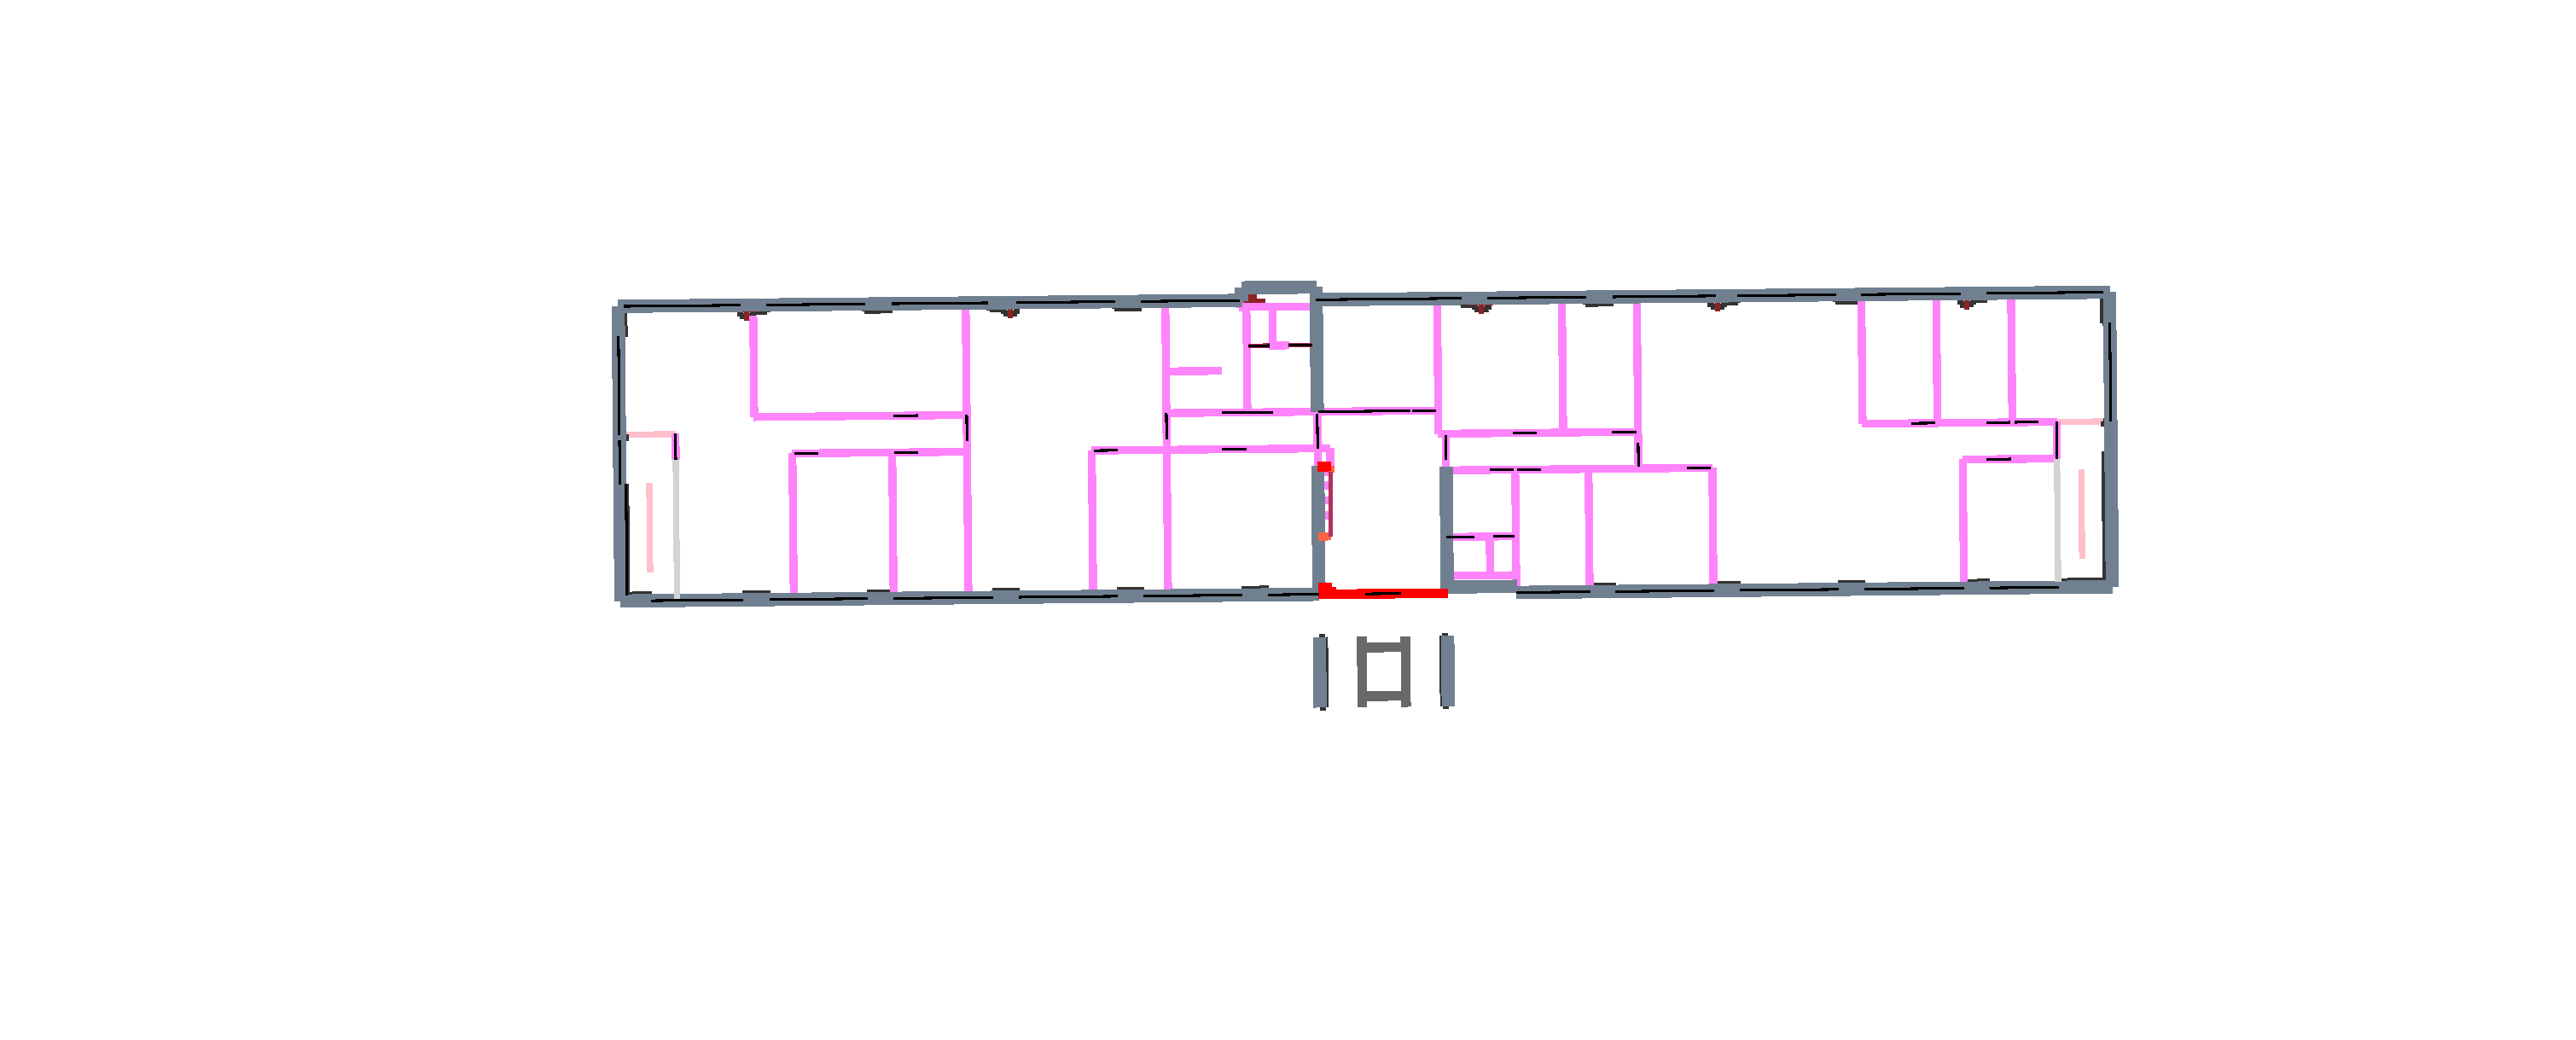
\includegraphics[width=7cm]{Gs2.pdf}
\caption{La légende est \emph{sous} la figure}
\end{centering}
\end{figure}
%






\begin{figure}[htbp]
\begin{centering}
\textsf{Une figure A single column figure goes here}
\par\end{centering}
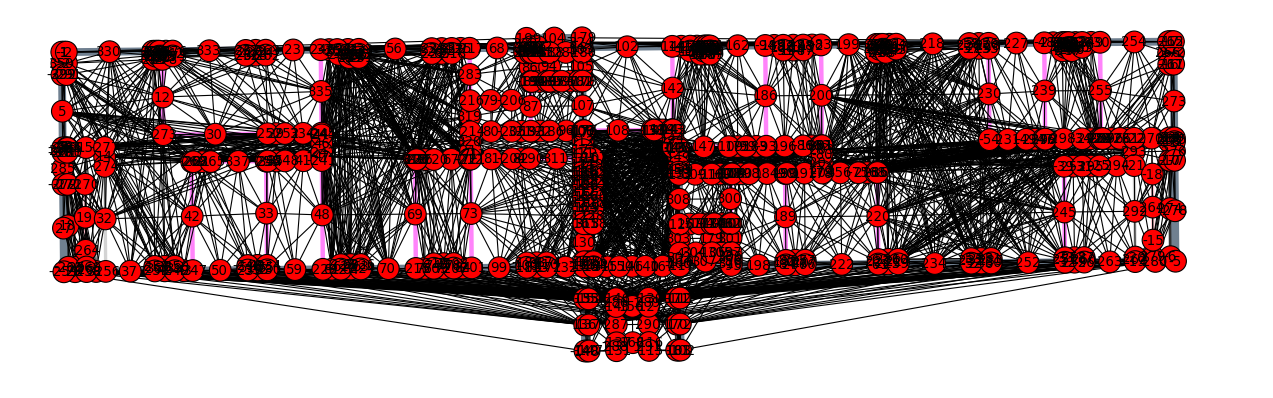
\includegraphics[width=7cm]{Gv.png}
\caption{La légende est \emph{sous} la figure}
\end{figure}
\begin{table}[htbp]
\caption{La légende  est \emph{sous} la table}


\centering{}
\begin{tabular}{|c|c|}
\hline 
delete & this\tabularnewline
\hline
\hline 
example & table\tabularnewline
\hline
\end{tabular}
\end{table}

\clubsuit
 

\section{Conclusions}

%
%\begin{comment}
%\bibliographystyle{IEEEbib}
\bibliographystyle{utphys}
%\bibliographystyle{alpha}
\bibliography{ref}

%\end{comment}
{}
\begin{biography}
{Votre Nom} All about you and the what your interests are. Don't
forget to put your name in between a pair of \{\}'s that are set as
raw \TeX{}.
\end{biography}

\begin{biography}
{Coauthor} Same again for the co-author.
\end{biography}

\end{document}
